
	\subsection{Uzajamno djelovanje naelektrisanih čestica}
	
	
	Elektrostatika je oblast fizike u kojoj se izučava elektricitet u mirovanju makroskopski posmatrano u odnosu na posmatračev referentni sistem, što znači da naelektrisanja smatramo statičkim (u miru) iako u njima postoji stalno kretanje naelektrisanih čestica.\\
	
	\begin{marginfigure}%
		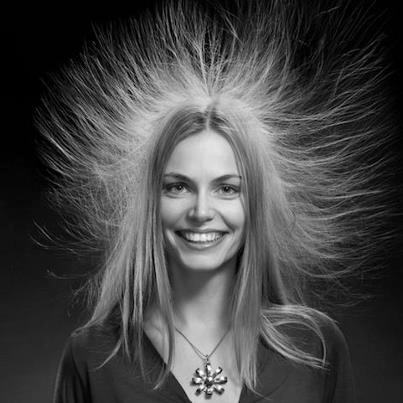
\includegraphics[width=\linewidth]{hair_static}
		\caption{Utvrđeno je da se neko tijelo može naelektrisati, ako se dodirne tijelom koje je već naelektrisano}
		\label{fig:hair_static}
	\end{marginfigure} 
	Fizikalna veličina koja opisuje stepen, odnosno mjeru naelektrisanosti neke čestice ili  tijela, zove se količina elektriciteta, količina naelektrisanja, ili električno opterećenje. Količina elektriciteta je skalarna, algebarska veličina, čija numerička vrednost govori, ili o višku, ili o manjku elektrona na nekom tijelu i označava se sa $ Q $ ili sa $ q $. Mjerna jedinica za količinu elektriciteta nosi naziv Kulon $ \textit{ C } $ francuskom fizičaru Kulonu.\\
	
	
	
	Rezultantno naelektrisanje atoma koji sadrži jednak broj protona i elektrona jednako je nuli. Kad neko tijelo sadrži višak elektrona, u odnosu na protone, kaže se da je negativno naelektrisano. U suprotnom, za tijelo koje ima manjak elektrona, kaže se da je pozitivno naelektrisano. Naelektrisanje $ q $, za koje se u literaturi susreću i nazivi: električno opterećenje, količina elektriciteta, električni naboj, jednako je:
	
	
	\begin{center}
		$ q= n e$,
	\end{center} 
	gdje je $ e $ elementarno naelektrisanje.
	%	\subsection{Elektroskop}

	\subsection{Elektroskop}
